\documentclass{beamer}
\usepackage{textcomp} %textrightarrow
\usepackage{listings}
\usepackage{graphicx}
\usetheme{Boadilla}
\title{Relazione lavoro svolto}
\author{Pietro Ghiglio}

\lstset{ 
  basicstyle=\footnotesize,        
  captionpos=none,                    
  commentstyle=\color{green},    % comment style
  extendedchars=true,              % lets you use non-ASCII characters; for 8-bits encodings only, does not work with UTF-8
  frame=single,	                   % adds a frame around the code
  keywordstyle=\color{blue},       % keyword style
  language=C,                 % the language of the code
  numbers=left,                    
  numbersep=5pt,                   
  numberstyle=\tiny\color{gray}, 
  rulecolor=\color{black},         
  stepnumber=1,                    
  tabsize=2,	                                 
}

\AtBeginSection[]
{
  \begin{frame}
    \frametitle{Table of Contents}
    \tableofcontents[currentsection]
  \end{frame}
}

\begin{document}
\titlepage

\begin{frame}
\frametitle{Table of Contents}
\tableofcontents
\end{frame}




\section{Instrumentazione}
\begin{frame}
\frametitle{Scopo}
\begin{itemize}
\item Propagare a livello di codice sorgente informazioni contenute tramite profiling.
\item Associare ad ogni riga di codice il numero di istruzioni provenienti da essa eseguite durante la run del programma. 
\item Associare ad ogni chiamata a funzione il numero di istruzioni eseguite a partire dalla chiamata.
\end{itemize}
\end{frame}

\begin{frame}
\frametitle{Implementazione}
\begin{itemize}
\item Stack di callsites, push prima di ogni chiamata, pop dopo la chiamata.
\item Ad ogni esecuzione di un basic block: stampa id basic block + dump dello stack. 
\end{itemize}
\end{frame}

\begin{frame}
\frametitle{Propagazione a livello di codice sorgente}
Dato un output dell'instrumentazione corrispondente all'esecuzione di un basic block: bbId callsite1 callsite2 ... callsiteN
\begin{itemize}
\item Per ogni istruzione llvm contenuta nel basic block corrispondente all'id, assegnare il costo dell'esecuzione dell'istruzione llvm alla location di codice sorgente corrispondente.
\item Per ogni callsite nel dump dello stack, assegnare il costo dell'istruzione llvm al callsite, a meno di funzioni ricorsive.
\end{itemize}
\end{frame}

\subsection{Funzioni ricorsive}

\begin{frame}
\frametitle{Call Graph}
\begin{itemize}
\item Grafo in cui ogni vertice è una funzione.
\item Un edge (v,u) rappresenta il fatto che la funzione v chiama u.
\item Label sugli edge con callsite.
\item Una call (v,u) è ricorsiva se u == v o se da u è possibile richiamare v. ( (v,u) è parte di un ciclo ).
\end{itemize}
\end{frame}





\begin{frame}
\frametitle{Esempio-1}
\lstinputlisting[language=C]{test3.c}
\end{frame}

\begin{frame}
\frametitle{Esempio-1}
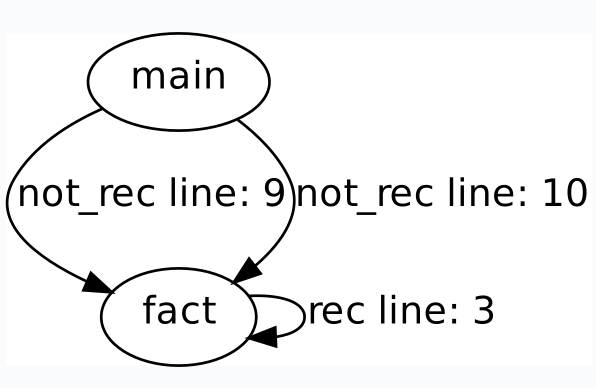
\includegraphics[scale=0.5]{graph3.png}
\end{frame}

\begin{frame}
\frametitle{Esempio-2}
\lstinputlisting[language=C, firstline=1, lastline=10]{test5.c}
\end{frame}

\begin{frame}
\frametitle{Esempio-2}
\lstinputlisting[language=C, firstline=11, lastline=23, firstnumber=11]{test5.c}
\end{frame}

\begin{frame}
\frametitle{Esempio-2}
\lstinputlisting[language=C, firstline=24,firstnumber=24]{test5.c}
\end{frame}


\begin{frame}
\frametitle{Esempio-1}
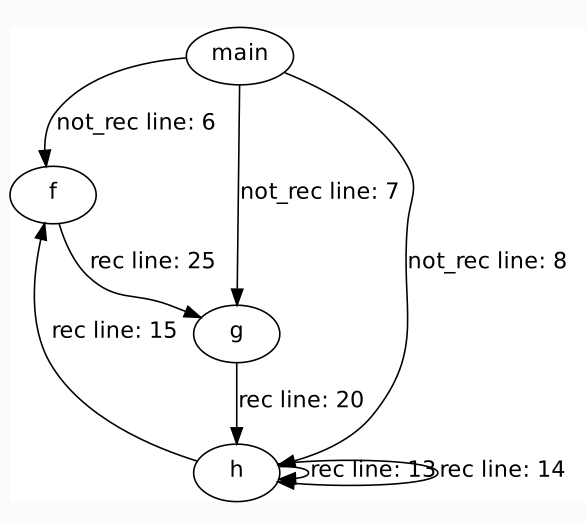
\includegraphics[scale=0.45]{graph5.png}
\end{frame}

\begin{frame}
\frametitle{Criterio di attribuizione}
Costo dell'istruzione attribuito al callsite solo se non è una chiamata ricorsiva.
\end{frame}


\section{Metriche}

\begin{frame}
\frametitle{Metriche utilizzate}

Al momento le metriche utilizzabili sono:
\begin{itemize}
\item Il numero di istruzioni LLVM: ogni istruzione LLVM ha costo 1. \item Il numero di istruzioni Assembly: ogni istruzione LLVM ha costo pari al numero di istruzioni assembly ad essa associato. 
\end{itemize}
Ad entrambe potrebbe essere associato un costo energetico o diretto (istruzioni LLVM) o dato dalla somma del costo delle istruzioni assembly corrispondenti. \linebreak
Richiede un energy model della target architecture, con le varie considerazioni sulla fattibilità in base alla complessità dell'architettura.

\end{frame}

\section{Mapping Source $\rightarrow$ LLVM $\rightarrow$ Assembly}
\begin{frame}
\frametitle{Mapping Source $\rightarrow$ LLVM}

Mapping source $\rightarrow$ LLVM direttamente dalle debug information delle API LLVM (classi DebugLoc, DISubProgram). \linebreak Alcune istruzioni (es. malloca all'inizio della funzione) non hanno debug info. In tal caso vengono attribuite alla line di definizione della funzione.


\end{frame}

\begin{frame}
\frametitle{Mapping LLVM $\rightarrow$ Assembly}
Mapping LLVM $\rightarrow$ Assembly ottenuto tramite un pass che sostituisce le informazioni di debug riguardo alla linea di codice sorgente con un id dell'istruzione stessa. \linebreak Molti metodi delle API LLVM per la modifica delle informazioni di debug sono privati. \linebreak Le informazioni di debug sostituite vengono recuperate effettuando disassembly dell'eseguibile.
\end{frame}

\section{Demo}

\begin{frame}
\frametitle{Codice}
\lstinputlisting{test3.c}
\end{frame}

\begin{frame}
\frametitle{CallGraph}
\lstinputlisting{test3.dot}
\end{frame}

\begin{frame}[fragile]
\frametitle{Disassembly pre fix}
\begin{verbatim}
name: main
begin: 401170 end: 40119e
addr: 401170 	pushq	%rbp debug: 8 
addr: 401171 	movq	%rsp, %rbp 
addr: 401174 	subq	$16, %rsp 
addr: 401178 	movl	$9, %edi debug: 31 
addr: 40117d 	callq	-114 
addr: 401182 	movl	$3, %edi debug: 32 
addr: 401187 	movq	%rax, -8(%rbp) 
addr: 40118b 	callq	-128 
addr: 401190 	xorl	%ecx, %ecx 
addr: 401192 	movq	%rax, -16(%rbp) 
addr: 401196 	movl	%ecx, %eax debug: 33 
addr: 401198 	addq	$16, %rsp 
addr: 40119c 	popq	%rbp 
addr: 40119d 	retq 
addr: 40119e 	nop debug: 33 
\end{verbatim}
\end{frame}

\begin{frame}[fragile]
\frametitle{Disassembly post fix}
\begin{verbatim}
name: main
begin: 401170 end: 40119e
addr: 401170 	pushq	%rbp debug: 31 
addr: 401171 	movq	%rsp, %rbp debug: 31 
addr: 401174 	subq	$16, %rsp debug: 31 
addr: 401178 	movl	$9, %edi debug: 31 
addr: 40117d 	callq	-114 debug: 31 
addr: 401182 	movl	$3, %edi debug: 32 
addr: 401187 	movq	%rax, -8(%rbp) debug: 32 
addr: 40118b 	callq	-128 debug: 32 
addr: 401190 	xorl	%ecx, %ecx debug: 32 
addr: 401192 	movq	%rax, -16(%rbp) debug: 32 
addr: 401196 	movl	%ecx, %eax debug: 33 
addr: 401198 	addq	$16, %rsp debug: 33 
addr: 40119c 	popq	%rbp debug: 33 
addr: 40119d 	retq debug: 33 
addr: 40119e 	nop debug: 33 
\end{verbatim}
\end{frame}

\begin{frame}[fragile]
\frametitle{Istruzioni LLVM}
\begin{verbatim}
31:   %1 = call i64 @fact(i32 9), !dbg !11
32:   %2 = call i64 @fact(i32 3), !dbg !12
33:   ret i32 0, !dbg !13
\end{verbatim}
\end{frame}

\begin{frame}
\frametitle{Attribuzione - LLVM}
\lstinputlisting{attr-llvm.c}
\end{frame}

\begin{frame}
\frametitle{Attribuzione - Assembly}
\lstinputlisting{attr-ass.c}
\end{frame}

\section{Conclusioni}
\begin{frame}
\frametitle{Come procedere ora?}
\begin{itemize}
\item Function mangling.
\item File multipli.
\item Energy model.
\item Ottimizzazioni del compilatore.
\item Chiamate a libreria.
\end{itemize}
\end{frame}




\end{document}